\chapter{Background}
\label{ch:background}

\section{Mesoscale Convective Systems in the Horn of Africa}

\acrfullpl{mcs} constitute a critical component of regional weather forecasting and climatology due to their significant size, duration, and impact. Officially, \acrshortpl{mcs} are defined as a complex of thunderstorms which become organised on a scale larger than any of the individual thunderstorms \citep{NOAANWS2025}. Consequently, these storm systems often last for several hours and cover areas of tens of thousands of square kilometres. In addition, they often produce severe weather phenomena, including flooding, strong winds, and hail \citep{Houze2014}. Unlike many \Gls{synopticscale} systems, \acrshortpl{mcs} are not usually associated with a well-defined centre of circulation and instead are characterised by their multi-scale organisation, typically incorporating a variety of convective cells and larger-scale features, such as squall lines or mesoscale convective complexes \citep{AMS2024,NOAANWS2025}. These systems are prevalent throughout the world and thus are key to understanding regional climatology. For example, in the United States, \acrshortpl{mcs} are a primary driver of warm-season precipitation over the Great Plains \citep{Haberlie2019}. Similarly, the Sahel region of Africa is heavily affected by these storms, producing some of the strongest \acrshortpl{mcs} globally due to it being a climatic transition zone with strong seasonal cycles \citep{Zipser2006}.

The Horn of Africa is a region with complex topography and large-scale climatic variability that affect \acrshort{mcs} development. As seen in Figure \ref{fig:horn-of-africa}, from the west, the Sahel fades into the Ethiopian Highlands and later the East African Rift Valley, characterised by high topographic relief and complex orography. In the east, the Ethiopian Highlands transition into the low-lying coastal plains of Somalia. Unlike other countries at this latitude, most of Somalia is arid or semi-arid, with the exception of its border region with Kenya \citep{Beck2023}. This contrast in geography is reflected in storm development and precipitation patterns. The mountains of Ethiopia dominate local convective processes \citep{Negash2024} while the low-lying areas on the south-eastern coast of the region are not nearly as conducive to \acrshort{mcs} development and thus are much more susceptible to storm patterns over the Indian Ocean and the Gulf of Aden \citep{Camberlin2024}. The combination of land surface temperature and soil moisture also impact the storm development and intensification. Notably, multiple studies over distinct regions have demonstrated that strong soil moisture gradients can intensify convection \citep{Barton2021,Klein2020,Taylor2017}. These processes are likewise relevant to the Horn of Africa, especially in transitional climates bridging arid and humid zones. Large-scale \glspl{teleconnection} also play a major role in governing \acrshort{mcs} activity in this region. The \acrfull{mjo} is a dominant intra-seasonal factor which modulates rainfall in the tropics and in East Africa, its active phases coincide with increased convection and extreme rainfall events \citep{Camberlin2019,Ochieng2023,Pohl2006}. Quite uniquely for the tropics, the \acrfull{itcz} passes over the region twice per year leading to two distinct rainy seasons, one short and one long \citep{Palmer2023,Tefera2025}. The \acrfull{tej} is another key feature enhancing vertical wind shear which can both facilitate or hinder \acrshort{mcs} development \citep{Farnsworth2011,Vashisht2021}. Additionally, the \acrfull{enso} and the \acrfull{iod} have also been shown to modulate rainfall patterns in the region, with coupled regional climate models able to reproduce these patterns at various timescales \citep{Dubache2019,Endris2019,Vashisht2021,Zaroug2014}. 

\begin{figure}[h]
    \centering
    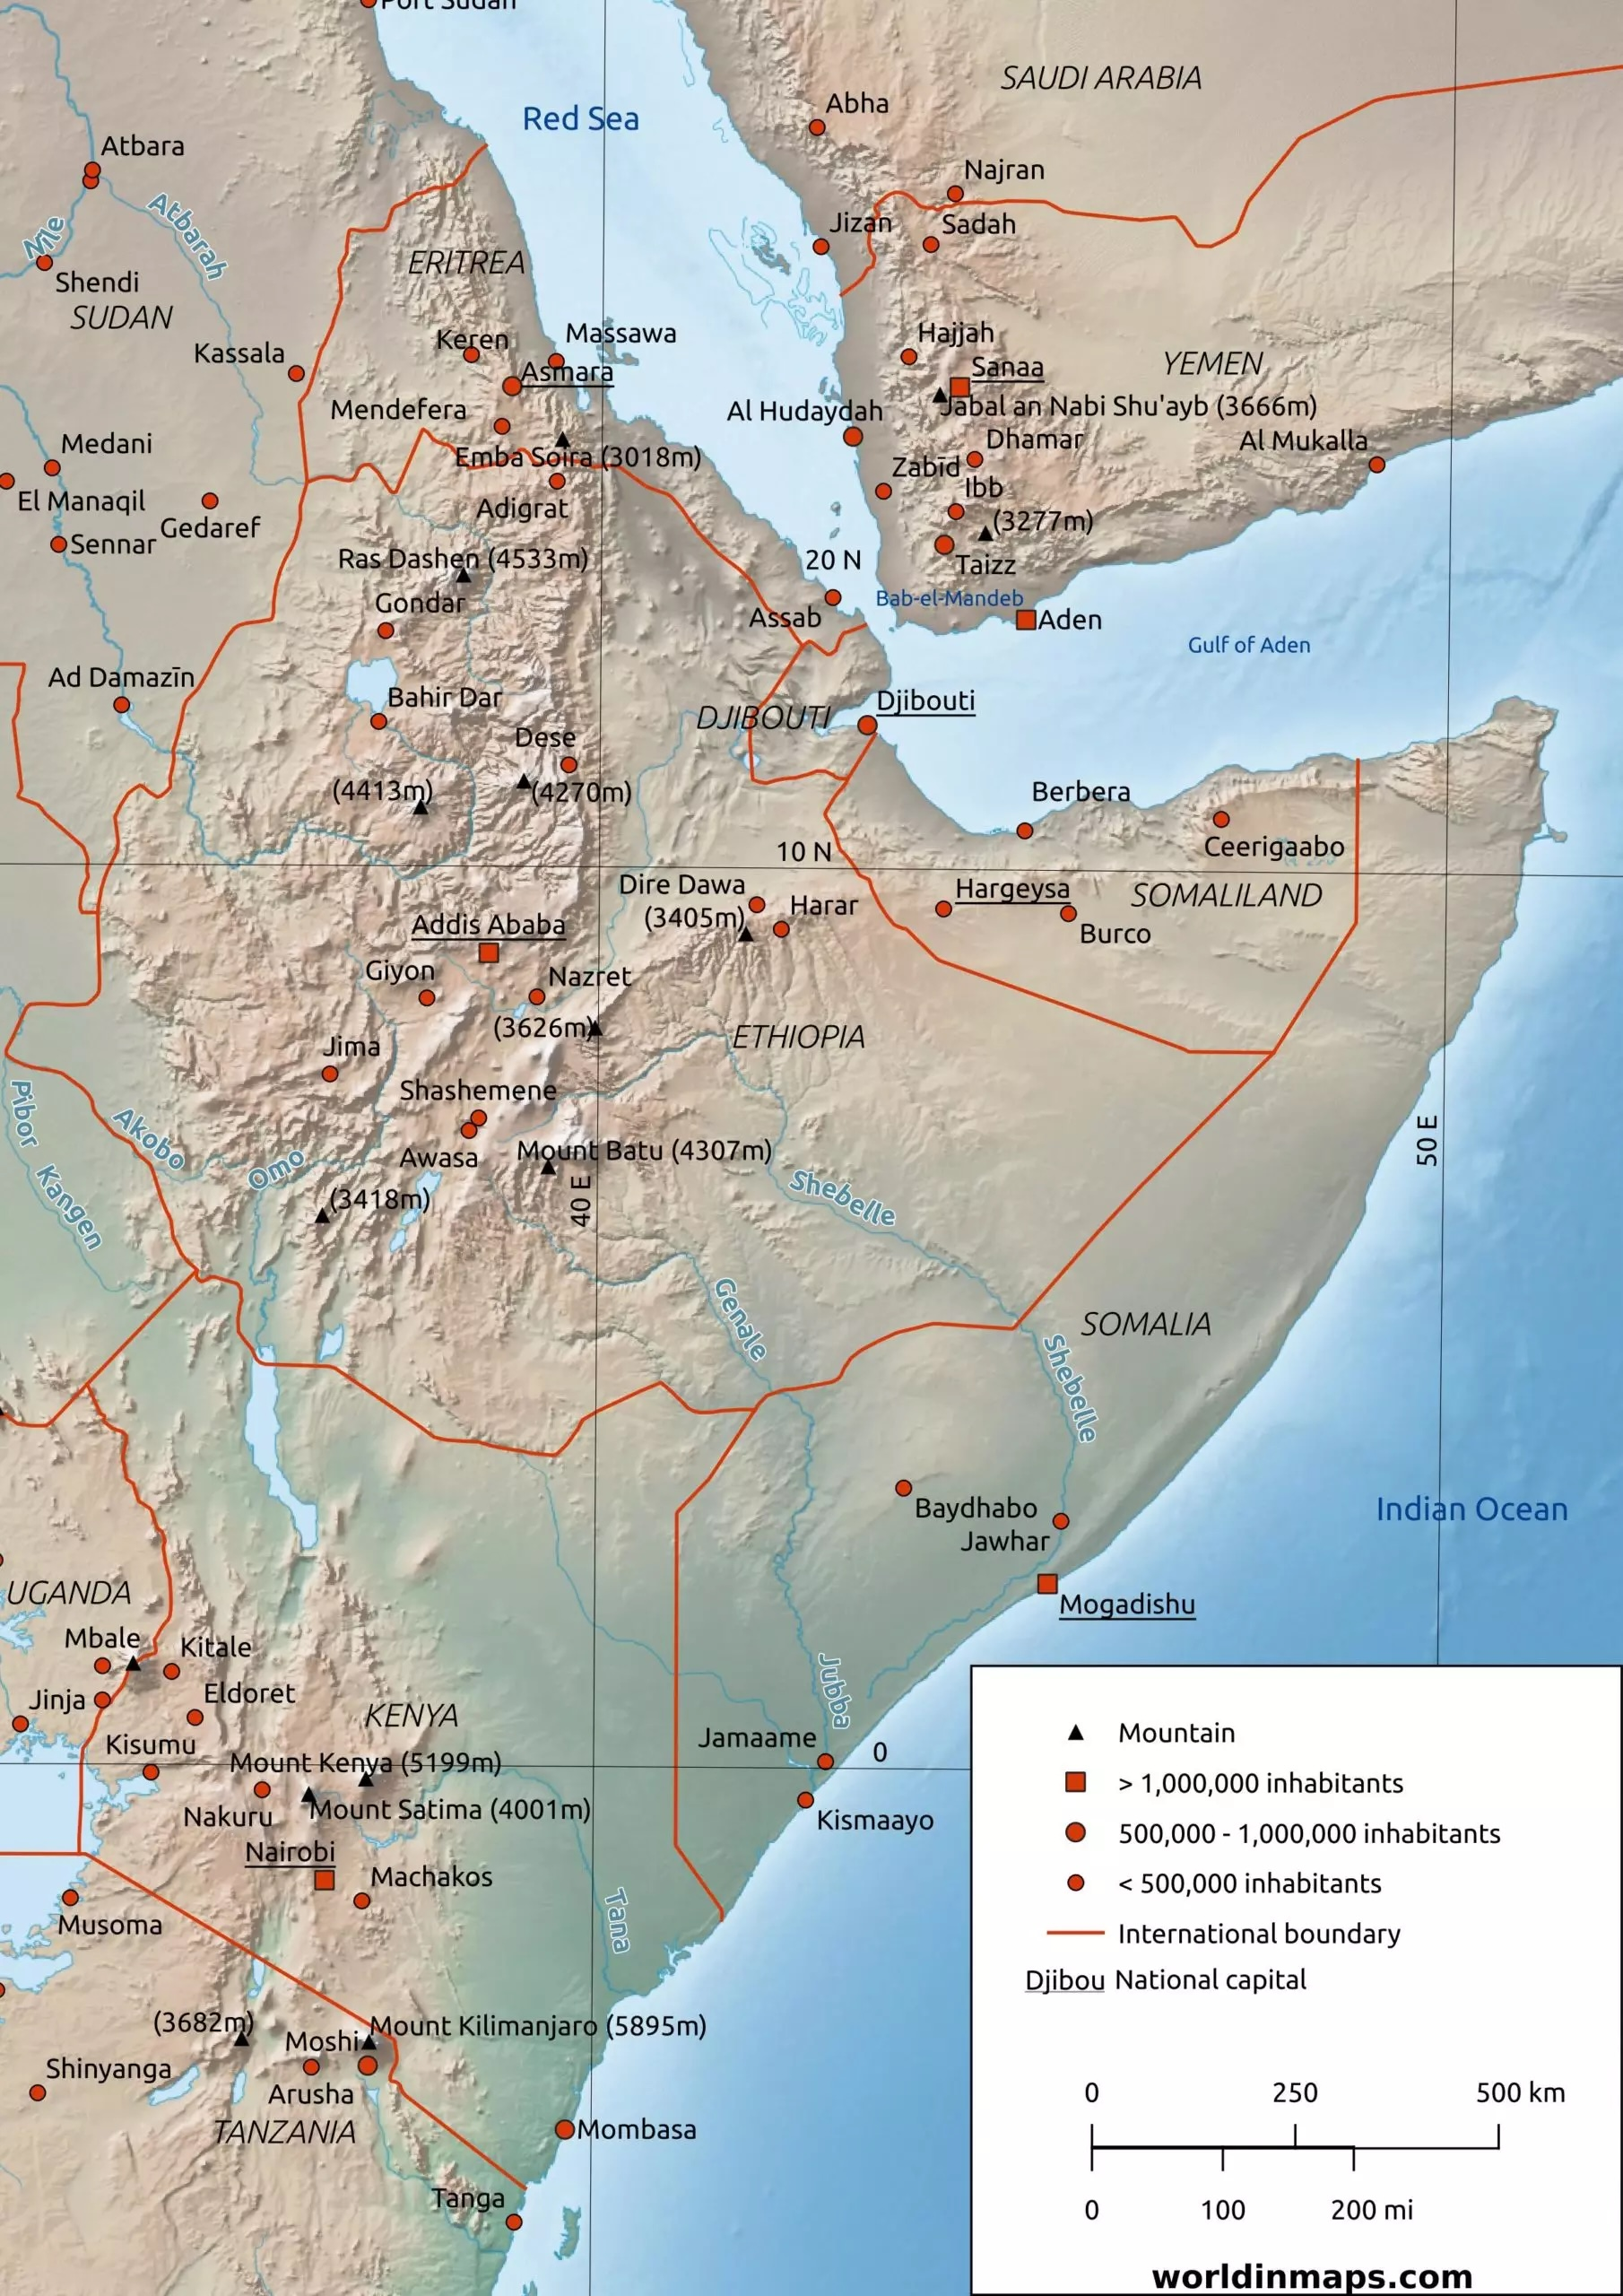
\includegraphics[width=0.6\textwidth]{../figures/static/horn-of-africa-map-scaled.jpeg}
    \caption{Map of the Horn of Africa \citep{WorldInMaps2024}}
    \label{fig:horn-of-africa}
\end{figure}

Overall, despite this complex array of factors, \acrshortpl{mcs} have been shown to account for over 60\% of extreme rainfall in Ethiopia and Somalia \citep{Hill2023}. These anomalous events often lead to intense flooding, which not only can affect the local population, but also countries as far as Egypt due to the Ethiopian Highlands being a watershed origin for countless rivers including the Blue Nile \citep{Legese2020,Zaroug2014}. Thus, the importance of understanding these storms, predicting their behaviour, and anticipating their effects cannot be overstated. But due to the long history of colonisation and underdevelopment, the entire continent of Africa is considerably underrepresented in high-quality meteorological data and many national meteorological services lack critical resources to more effectively monitor and predict \acrshortpl{mcs} \citep{Dinku2019,Kinyondo2018,Meque2021}. This discrepancy also has downstream effects on global meteorology, as reanalysis datasets and digital twin systems rely heavily on data assimilation of observations and regional models for calibration abd parametrisation \citep{Linsenmeier2023,Valmassoi2023}. Although the primary remedy would be increased investment and study, this discrepancy presents an opportunity for otherwise unorthodox methods to make use of existing data to improve predictions and understanding of \acrshortpl{mcs}.

\section{Data-driven Scientific Discovery}

Although scientific research is no stranger to the analysis of experimental data to confirm hypotheses, since the advent of computers in the 20th century, the possibility of data-driven discovery has gained traction. The physical sciences have traditionally favoured numerical methods for complex system modelling, employing the resultant equations from first principles and physical laws as the basis for simulation. Since most of these systems are too complex to be solved analytically, numerical methods are used to approximate solutions within certain constraints limiting grid resolution, stability, and sub-grid processes \citep{Lynch2008}. The primary benefit of such techniques is their foundation on well-established physical laws by design which naturally provides a degree of trustworthiness. However, these methods famously struggle with the chaotic nature of many physical systems, particularly in meteorology where small changes can lead to vastly different outcomes \citep{Lorenz1963}. Other fields, such as biology and social sciences, also rely on computer simulations, but tend to favour statistical approaches for experimental hypothesis testing. Techniques for subsequent data analysis include linear regression, dimensionality reduction, and Bayesian inference \citep{Ackermann2011,Weinstein2010}. While these techniques would undoubtedly be considered subcategories of \acrshort{ml}, the tools remain largely supplemental to the dominant research methodologies.

In contrast, principally data-driven discovery methods have historically been avoided due the lack of data and computational infeasibility, even when such methods were known and their potential well-understood \citep{Rosenblatt1957,Rumelhart1986}. However, the advent of large datasets and ever-increasing computational power as hardware manufacturers kept pace with \Gls{mooreslaw} has led to a resurgence of interest in data-driven methods \citep{Haber2025}. Particular credit can be attributed to the surprise success of \acrfull{dl} in computer vision and natural language processing, which has led to a broader acceptance of advanced \acrfull{ml} techniques across many scientific disciplines \citep{Haber2025,Krizhevsky2017}. The key challenge remains the integration of these data-driven methods with existing scientific knowledge and frameworks as this requires not only advances in algorithmic design but also domain expertise. However, it is only a matter of time as more funding and effort are applied. In drug development, \acrfull{ml} appears to be revolutionising the current search for the secrets of protein folding \citep{Jumper2021}, while the application of \acrshort{dl} to quantum phase transitions has reached parity with traditional methods and significantly less compute \citep{Huembeli2018}.

The field of meteorology has been no exception to the increasing popularity of data-driven methods, with a growing body of literature exploring the application of \acrshort{ml} techniques to various meteorological problems. Ample amounts of manual observations spanning nearly centuries, petabytes of satellite imagery since the early 1990s, and the output of numerical models from national forecast offices worldwide, constitute a formidable treasure trove for training and validating these models \citep{Bracco2024,Waqas2024,Zhang2025}. Given the profound complexity of atmospheric processes, there are numerous opportunities at varying scales to improve our understanding and prediction of weather and climate phenomena. On the smaller scale, \acrshort{ml} has been used for tasks such as downscaling, parametrisation, and nowcasting, where the goal is to improve the resolution and accuracy of existing numerical forecasts \citep{Blunn2024,Zhang2023}. On the larger scale, reanalysis datasets like the \acrfull{ecmwf}'s \acrfull{era5} and \acrfull{nasa}'s \acrfull{merra2} have enabled the development of global models that can predict large-scale weather patterns with the partial goal of matching the performance of \acrfull{nwp} models \citep{Bracco2024,Gelaro2017,Hersbach2020,Zhang2025}.

In spite of the rapid emergence and success of these methods, the fundamental challenge of trustworthiness remains. The immense complexity of \acrshort{ml} algorithms, especially more recent \acrshort{dl} approaches, hastened the usage of the term \gls{blackbox} to describe how model behaviour is often nearly intractable. This could be particularly detrimental for meteorological applications, where the consequences of incorrect predictions can be severe. As a result, there is a growing interest in developing methods for explainable and interpretable \acrshort{ml}, known as \acrfull{xai}, to provide insights into the decision-making processes of these models \citep{Molnar2025}. An especially popular approach is to incorporate physical constraints and knowledge into the training process, usually directly in the architecture or loss function, incentivising the models to adhere to the laws of physics known to govern atmospheric processes \citep{Dabrowski2020,Chen2022,Luo2025,Zhang2023}. Referred to as \acrfull{piml}, this approach has shown promise in improving model performance and physical accuracy, but concerns still remain regarding interpretability and long-tail events in training data \citep{Lukacz2024,Radford2025,Sun2025}. Regardless, even while many seasoned meteorologists remain skeptical, it is clear that the integration of \acrshort{ml} into meteorology is a rapidly evolving field with significant potential.

\section{Explainable Artificial Intelligence}

\acrfull{xai} is an emerging field focused on developing methods and techniques to make the decision-making processes of \acrshort{ml} solutions more transparent and interpretable. This is particularly important in domains where understanding the rationale behind predictions is crucial, such as healthcare, finance, and meteorology \insertref{XAI in these fields}. Approaches in this field take a variety of forms, including inherently interpretable models and post-hoc explanation methods. A summary of \acrshort{xai} taxonomy is given in Figure \ref{fig:xai-taxonomy}.

\begin{figure}[h]
    \centering
    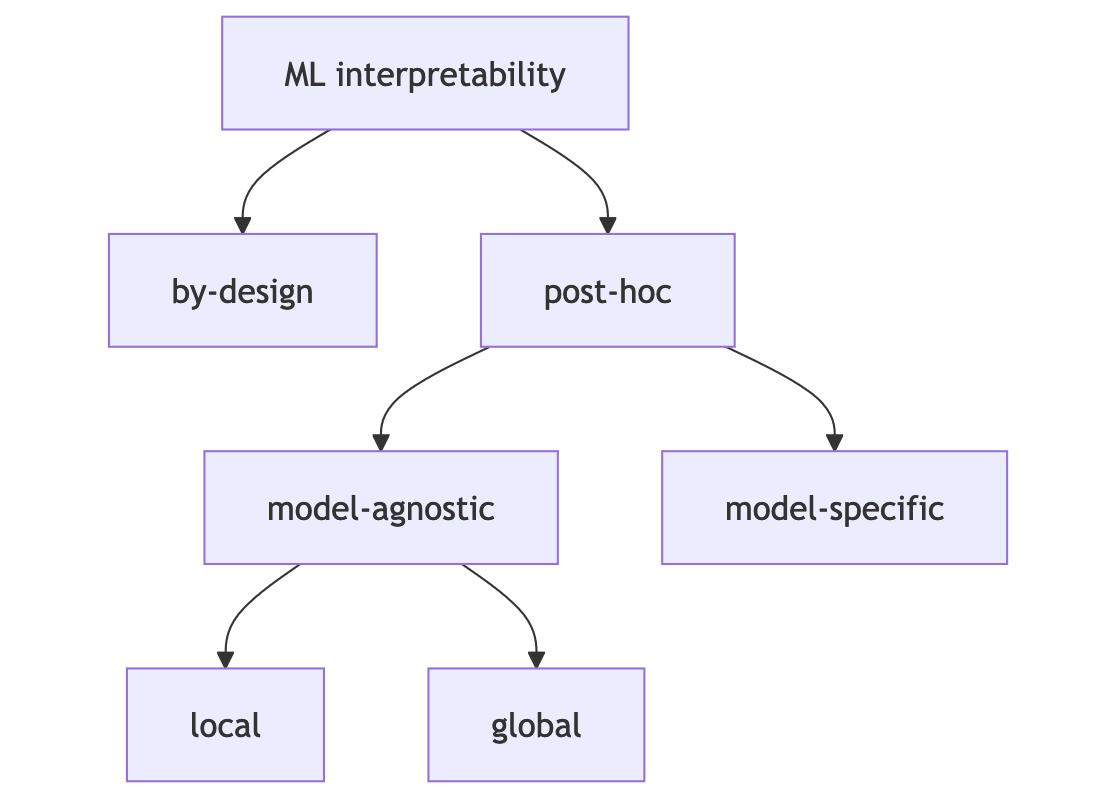
\includegraphics[width=0.8\textwidth]{../figures/static/xai-taxonomy.jpg}
    \caption{XAI Taxonomy (Figure 4.1 from \cite{Molnar2025})}
    \label{fig:xai-taxonomy}
\end{figure}

Inherently interpretable models are designed to be transparent by construction, often using simpler architectures or feature-based approaches that allow for direct interpretation of the relationship between inputs and outputs. Examples include linear regression, decision trees, and rule-based systems. A clear disadvantage is that these simpler models may sacrifice some predictive performance compared to more complex ones like \acrfull{dnn}. \acrshort{piml} could also be considered a part of this landscape, as it aims to integrate existing physical knowledge into architectures and training processes to enhance forecast accuracy and credibility. Post-hoc explanation methods, on the other hand, are applied to models after training to partially interpret their behaviour. Model-specific post-hoc methods directly leverage the learned structure of the model. For example, great strides have been made in pinning the internal embeddings and attention mechanisms of transformer models to real-world entities and concepts \citep{Lin2023}. Notably for this research, model-agnostic methods are predominantly designed to make no assumptions as to underlying model architecture. These methods can then be broadly categorised into local and global explanations. Local explanations focus on providing insights into model behaviour around a given input. In contrast, global explanations aim to provide an overall understanding of the model's behaviour for any input. For local explanations, counterfactual analysis has gained traction, especially for classification tasks, where the model's local decision boundary can be more interactively explored through slight perturbations of the a given input \citep{Mothilal2019}. \acrfull{shap} are both applicable for local and global explanations and will be used extensively throughout this research. As such, a brief overview of the approach follows.

\subsection{Shapley Additive Explanations}

After its popularisation via \cite{Lundberg2017} and the accompanying \texttt{shap} \texttt{python} library, \acrfull{shap} has emerged as one of the most prominent frameworks for post-hoc explainability. This is achieved through the application of coalitional game theory where the algorithm approximates a fair distribution of "payout", in this case a fraction of the model's prediction, among the input features based on their individual contributions to the prediction \citep{Shapley1953}. Formally, the Shapley value for a feature is calculated via the average marginal contribution of that feature across all possible coalitions of features weighted by the probability of the coalition, where a coalition is a subset of features, and the marginal contribution of a feature to a coalition is the difference in the model's prediction when that feature is included versus when it is excluded. This process ensures that each feature's contribution is fairly evaluated by accounting for its interactions with other features. The result is a set of Shapley values for each feature and model output, which can then be used to interpret the model's predictions locally, by highlighting the most influential features for a single output, or globally, by aggregating the Shapley values across multiple predictions to identify overall feature importance.

In practice, this algorithm experiences a \gls{combinatorialexplosion} as features increase, thus, various approximations and optimisations have been developed to make it feasible for larger datasets. For example, \cite{Lundberg2017} present a kernel-based method which operates on the assumption that not all coalitions are equally important in quantifying a features marginal contribution. The application of Shapley values for explaining \acrshort{ml} models was first proposed by \cite{trumbelj2011}, but \cite{Lundberg2017} key contribution was the introduction of an additive feature attribution model, which allows for efficient approximation using a linear model. This approach assumes that the prediction can be expressed as a sum of the feature contributions, making it easier to interpret and visualise. The \texttt{shap} library implements both model-specific and agnostic methods using this framework and provides various tools for visualising Shapley values and their impact on individual predictions and overall model performance.

\subsection{Review of Explainable Artificial Intelligence in Meteorology}

As the \acrshort{ml} techniques increasingly permeate the field of meteorology, the need for \acrshort{xai} is paramount if operational deployment is to be successful and trustworthy.

Main surveys:
\begin{itemize}
    \item \href{https://www.sciencedirect.com/science/article/pii/S1352231024004722}{Interpretable machine learning for weather and climate prediction: A review}
    \item \href{https://link.springer.com/chapter/10.1007/978-3-031-04083-2_16#Sec2}{Explainable Artificial Intelligence in Meteorology and Climate Science: Model Fine-Tuning, Calibrating Trust and Learning New Science}
\end{itemize}

\begin{itemize}
    \item LIME has helped identify crucial features in random forest models for seasonal precipitation prediction, with explanations aligning closely to known meteorological phenomena like ENSO impacts \insertref{\href{https://www.sciencedirect.com/science/article/abs/pii/S1352231024004722}{source}}.
    \item SHAP has been used to interpret the predictions of deep learning models for Tropical Cyclone Wind Radius, revealing the importance of environmental factors like sea surface temperature and vertical wind shear \insertref{\href{https://journals.ametsoc.org/view/journals/mwre/151/2/MWR-D-22-0166.1.xml}{source}}.
    \item 
\end{itemize}

\subsection{Explainable Artificial Intelligence for Convective Systems}

\begin{itemize}
    \item Layer-wise Relevance Propagation (LRP) in Tropical Cyclone Intensity and Size Estimation \insertref{\href{https://www.scopus.com/pages/publications/851092020842}{source}}.
    \item Paleoclimate reconstruction of Indian monsoon: \insertref{\href{https://cp.copernicus.org/articles/21/1/2025/}{source}}.
    \item Predicting rainfall extremes in Africa: \insertref{\href{https://www.sciencedirect.com/science/article/abs/pii/B9780443288678000046}{source}}.
    \begin{itemize}
        \item not explicitly XAI, but they did use interpretable models like xgboost
    \end{itemize}
\end{itemize}

The main inspiration for the methodology employed in this thesis comes from \cite{Hunt2024}'s investigation of interpretable gradient-boosted decision-trees for uncovering dynamical relationships governing \gls{indianmonsoon} \acrfull{lps}. They first utilise a tracking algorithm to assemble a database of \acrshort{lps} storm tracks from \acrshort{era5} data. Using the storm centroids along each track, they extract a set of meteorological features from the surrounding \acrshort{era5} data as well as invariant but meaningful features like orographic elevation under the centroid. These features are then used to train a gradient-boosted decision tree model to predict specific storm characteristics, like mean precipitation or peak vorticity. The model is then interpreted using \acrshort{shap} values to not only identify the most important features, but also reveal how feature importance changes relative to geography. The authors posit several notable results including the observation that processes affecting intensification differ from those affecting peak intensity and also confirm existing research that mid-level winds are relevant for predicting storm speed and direction. This methodology is particularly compelling as it also offers a framework that could be adapted for other regions and storm types with the only pre-requisite being high quality storm track data. Such data does already exist in some cases (e.g. the European Windstorm Catalogue \citep{Roberts2014}), but \cite{Hunt2024} show that, for certain storm types, the tracks can be derived from reanalysis data.

However, there are also many additional avenues for exploration, especially leveraging the explanatory power of \acrshort{shap} values. For example, \cite{Hunt2024} primarily focus on the model's ability to capture the relationships between features and storm characteristics, but do not explore the model's ability to predict storm tracks or propagation. While interpretable \acrshort{ml} techniques pale in comparison to traditional \acrfull{nwp} models, their insights may be able to aid with sub-grid parametrisation or facilitate the planning of new observational networks in data-scarce and computationally limited regions like Africa. Furthermore, while \cite{Hunt2024} do take great care to justify the inclusion of each feature and remove those that are highly correlated, they do not explore the possibility of direct comparison between models trained with different feature sets. This could be useful in disentangling the relative importance of meteorological and geographical features, which may often work in concert or direct opposition, such as wind angle and orography. Thus, this thesis aims to build upon their work by exploring these additional avenues and further investigating the potential of interpretable \acrshort{ml} techniques for understanding and predicting storm behaviour.